\documentclass[../main.tex]{subfiles}

\begin{document}

Si consideri ora un network generato dalla matrice di adiacenza simmetrica $\mathcal{A}_{ij}$ i cui nodi rappresentano gli incroci di una rete stradale.
Alla matrice di adiacenza \`e associata una matrice dei pesi $\mathcal{S}_{ij} \geq 0$ che, associando un diverso peso ad ogni link, definisce la lunghezza delle strade.
Su questo network si definiscano ora le classi di agenti $C_{1},\ldots,C_{k}$, ognuna delle quali caratterizzata da un nodo sorgente $s$ e destinazione $d$ e denotate come $C_{\alpha}(s,d)$.
Ogni individuo dovr\`a, nel corso della simulazione, muovere tra i nodi $s\to d$ in modo da seguire la geodetica, ossia il percorso pi\`u breve.
Il costo di un percorso, tuttavia, non viene calcolato sulla base della lunghezza: data la mobilit\`a dei veicoli, risulta pi\`u accurato considerando il tempo di percorrenza.
A tale fine si definisca ora un'altra matrice dei pesi $\mathcal{V}_{ij} \geq 0$ rappresentante la velocit\`a massima alla quale un agente pu\`o andare su una determinata strada.
L'elemento di matrice
\begin{equation}
    \mathcal{T}_{ij}=
    \begin{cases}
        \frac{\mathcal{S}_{ij}}{\mathcal{V}_{ij}} \quad& \mathcal{V}_{ij} \neq 0\\
        0 \quad& \mathcal{V}_{ij} = 0
    \end{cases}
\end{equation}
rappresenta dunque il costo temporale associato al link $i \to j$.\\
Discretizzando il tempo con un passo $\Delta t$, si \`e ora interessati a calcolareil costo di un percorso.
Considerando un path generico a $k$ step $A^{c} = \left\{a_{1} \to a_{2} \to \ldots \to a_{c}\right\}$, con $a_{0} = s$ e $a_{c} = d$, il costo del percorso \`e esprimibile come
\begin{equation}
    G=c\Delta t
\end{equation}
dove $c \in \mathbb{N}$.
Nel limite di individui non interagenti tra di loro \`e quindi possibile calcolare costo della geodetica, chiamata \emph{best path}, come
\begin{equation}
    G_{\text{best}} = c_{\text{best}}\Delta t = \min_{A^{c}} \left\{\sum_{i=1}^{c-1}\mathcal{T}_{i,i+1}\right\}
    \label{eq:best_path}
\end{equation}
Questo limite risulta molto stringente, in quanto nella realt\`a ogni veicolo presente sulla strada \`e evidentemente influenzato dalla presenza degli altri.
Tuttavia, lo scopo del modello \`e l'analisi macroscopica delle congestioni, quindi dettagli microscopici come questo si sono potuti trascurare.
Si assuma ora che gli agenti muovano sulla rete seguendo un moto stile random walk.
Per ogni classe di individui $C_{\alpha}$ \`e quindi necessario definire una matrice stocastica (di transizione) $\pi_{ij}^{\alpha}$ con le propriet\`a descritte nella sezione precedente.
Nella realt\`a una strada ha una capacit\`a finita, intesa come numero massimo di veicoli presenti su di essa in un generico istante di tempo $t$.
Tale vincolo viene implementato nel modello tramite l'introduzione di una densit\`a massima $\rho_{max}$ caratteristica di ogni strada: questa dipender\`a, naturalemente, sia dalla lunghezza della strada che dalla lunghezza dei veicoli cicolanti su di essa.
Assumendo la lunghezza media dei veicoli sia un valore fissato $\bar{l}_v$ e la lunghezza di una strada generica sia $l_s$, la densit\`a massima \`e calcolabile come
\begin{equation}
    \rho_{max}=\frac{\bar{l}_v}{l_s}
    \label{eq:density}
\end{equation}
Si osservi come il valore di $l_s$ sia sempre noto, essendo un elemento della matrice $\mathcal{S}$.

\section{Algoritmo di evoluzione}
\`E ora necessario definire come i veicoli muovano effettivamente sul network.
La probabilit\`a di transizione di osgni classe $\pi_{ij}^{\alpha}$ viene assegnata nel modo seguente:
\begin{itemize}
    \item fissato il nodo di partenza $i$ si inizia a scorrere sul passo successivo nel nodo $j$;
    \item se il nodo $j$ si trova sul percorso $G_{\text{best}}$, definito dall'Eq. (\ref{eq:best_path}), allora viene assegnato un peso $\pi_{ij}=1$;
    \item altrimenti, se il link esiste ($\mathcal{A}_{ij} \neq 0$) viene assegnato un peso $\pi_{ij}=\tanh \beta T$, dove $\beta$ \`e un parametro di controllo del modello e $T$ rappresenta una temperatura statistica;
    \item una volta controllati tutti i possibili $j$ il vettore riga $i$-esimo viene poi normalizzato in modo tale da avere $\sum_j\pi_{ij}=1$.
\end{itemize}
Si osservi che grazie all'introduzione della temperatura statistica $T$, graficata in Fig. \ref{fig:temperature}, \`e possibile permettere agli agenti di ``sbagliare'' percorso e uscire dalla geodetica, introducendo cos\`i delle fluttuazioni.
Inoltre, per $T \to \infty$ l'evoluzione del sistema diventa equivalente ad un random walk su network in quanto ogni scelta di percorso ha la medesima probabilit\`a.
\begin{figure}[H]
    \centering
    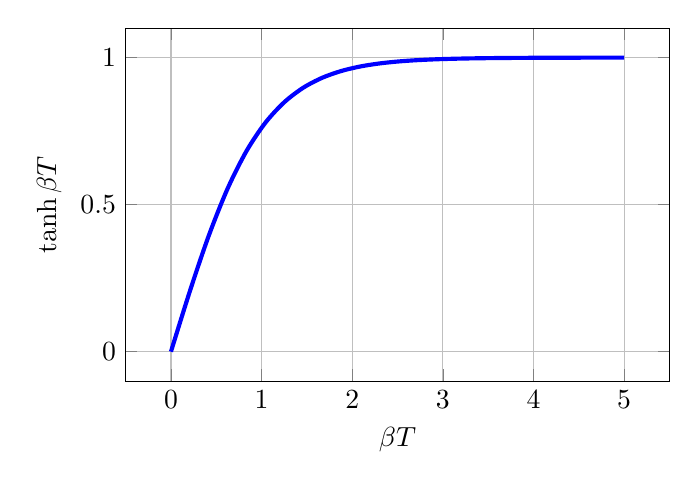
\begin{tikzpicture}
        \begin{axis}[
            grid = both,
            major grid style = {lightgray},
            minor grid style = {lightgray},
            width = 0.7\textwidth,
            height = 0.5\textwidth,
            xlabel = {$\beta T$},
            ylabel = {$\tanh \beta T$},]
            \addplot[
                domain = 0:5,
                smooth,
                color = blue,
                line width = 1.5pt,] {tanh(x)};
        \end{axis}
    \end{tikzpicture}
    \caption[Temperatura statistica]{\emph{Probabilit\`a di errore in funzione della temperatura statistica.}}
    \label{fig:temperature}
\end{figure}
Considerando ora un individuo generico appartente alla classe $C_{\alpha}$ si procede nel modo seguente:
\begin{itemize}
    \item si controlla se sia in grado di muoversi, quindi se $c = 0$. In caso negativo si sconta uno step temporale $c = c -1$ e si prosegue con gli altri veicoli;
    \item in caso affermativo, il passo successivo sarà deciso stocasticamente dalla matrice $\pi_{ij}^{\alpha}$;
    \item se la strada di arrivo \`e piena si perde uno step temporale, altrimenti l'individuo si immette sulla strada che connette i nodi $i \to j$ regolando la sua velocit\`a secondo la legge 
    \begin{equation}
        v(t) = v_{max}\left(1-k\frac{\rho(t)}{\rho_{max}}\right)
        \label{eq:velocity}
    \end{equation}
    dove $\rho(t)$ rappresenta la densit\`a di veicoli presenti sulla strada al tempo $t$ e $k$ \`e un parametro di controllo del modello;
    \item in base alla velocit\`a acquisita all'inviduo viene poi assegnata una nuova penalit\`a temporale $c = \frac{L}{v(t)\Delta t}$, con $L$ lunghezza della strada in cui si trova.
\end{itemize}
\begin{figure}[H]
    \centering
    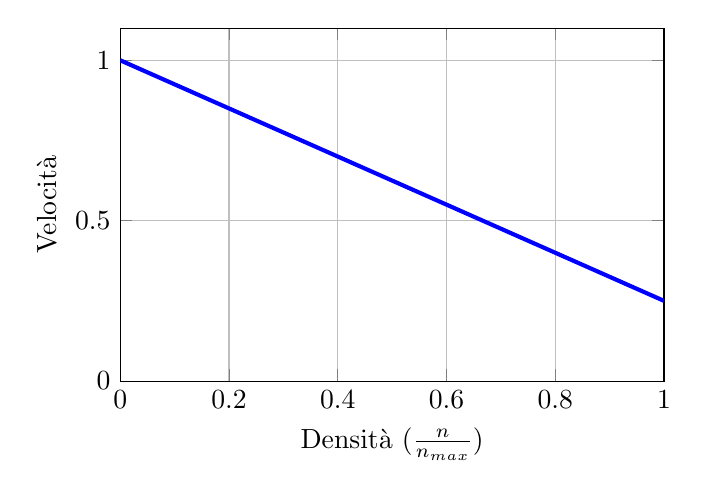
\begin{tikzpicture}
        \begin{axis}[
            grid = both,
            major grid style = {lightgray},
            minor grid style = {lightgray},
            ymin=0,
            xmin=0,
            xmax=1,
            width = 0.7\textwidth,
            height = 0.5\textwidth,
            xlabel = {Densità ($\frac{n}{n_{max}}$)},
            ylabel = {Velocità},]
        \addplot[
            domain = 0:1,
            smooth,
            color = blue,
            line width = 1.5pt,] {1-0.75*x};
        \end{axis}
    \end{tikzpicture}
    \caption[Velocit\`a nel modello]{\emph{Ipotesi dell'andamento della velocit\`a in funzione della densit\`a per $k = 0.75$.}}
    \label{fig:velocity}
\end{figure}
Si noti come l'Eq. (\ref{eq:best_path}), graficata in Fig. \ref{fig:velocity}, tenda all'ipotesi di Greenshield per $k = 1$ (cfr. Eq. (\ref{fig:greenshield})).

\section{Parametri di controllo}
Durante la costruzione del modello sono emersi alcuni parametri da cui esso dipende che vengono esplicitamente richiesti in input.
Questi sono:
\begin{itemize}
    \item \emph{Lunghezza media dei veicoli}, rappresentata dal parametro $\bar{l}_v$ presente in Eq. (\ref{eq:density}).
        Si nota immediatamente come la densit\`a massima sulle strade dipenda da esso e, di conseguenza, anche flusso e densit\`a (cfr. Eq. (\ref{fig:greenshield}));
    \item Coefficiente $k$ della temperatura statistica, rappresenta il grado di crescita delle fluttuazioni statistiche presenti nel sistema;
    \item \emph{Velocit\`a minima su una strada}, rappresenta la velocit\`a corrispondente alla densit\`a massima, come espresso in Eq. (\ref{eq:velocity}).
        Da questa dipender\`a naturalmente l'evoluzione temporale del sistema stesso;
    \item \emph{Flusso di veicoli immessi}, ossia il numero di veicoli immessi nella rete per unit\`a di tempo;
    \item \emph{Tempo di esecuzione}, il quale deve essere impostato in base al tipo di fenomeno che si vuole osservare.
\end{itemize}
Naturalmente la simulazione dipende dalle caratteristiche geometriche del sistema, come la rete stessa (inserita come matrice di adiacenza) e le classi di veicoli.

\begin{itemize}
    \item \emph{Lunghezza media dei veicoli}
\end{itemize}


\end{document}